\documentclass{article}
\usepackage{graphicx}

\title{Resume Video Oracle}
\begin{figure}
    \begin{center}
        
\includegraphics[width=6cm]{poltekpos.jpg}
    \end{center}
\end{figure}
\author{Annisa Khairani Febrianti}
\date{1184071}

\begin{document}

\maketitle

\section{Video Oracle Apex}
\begin{enumerate}
    \item Pertama klik app builder
    \begin{figure}[h]
            \centerline{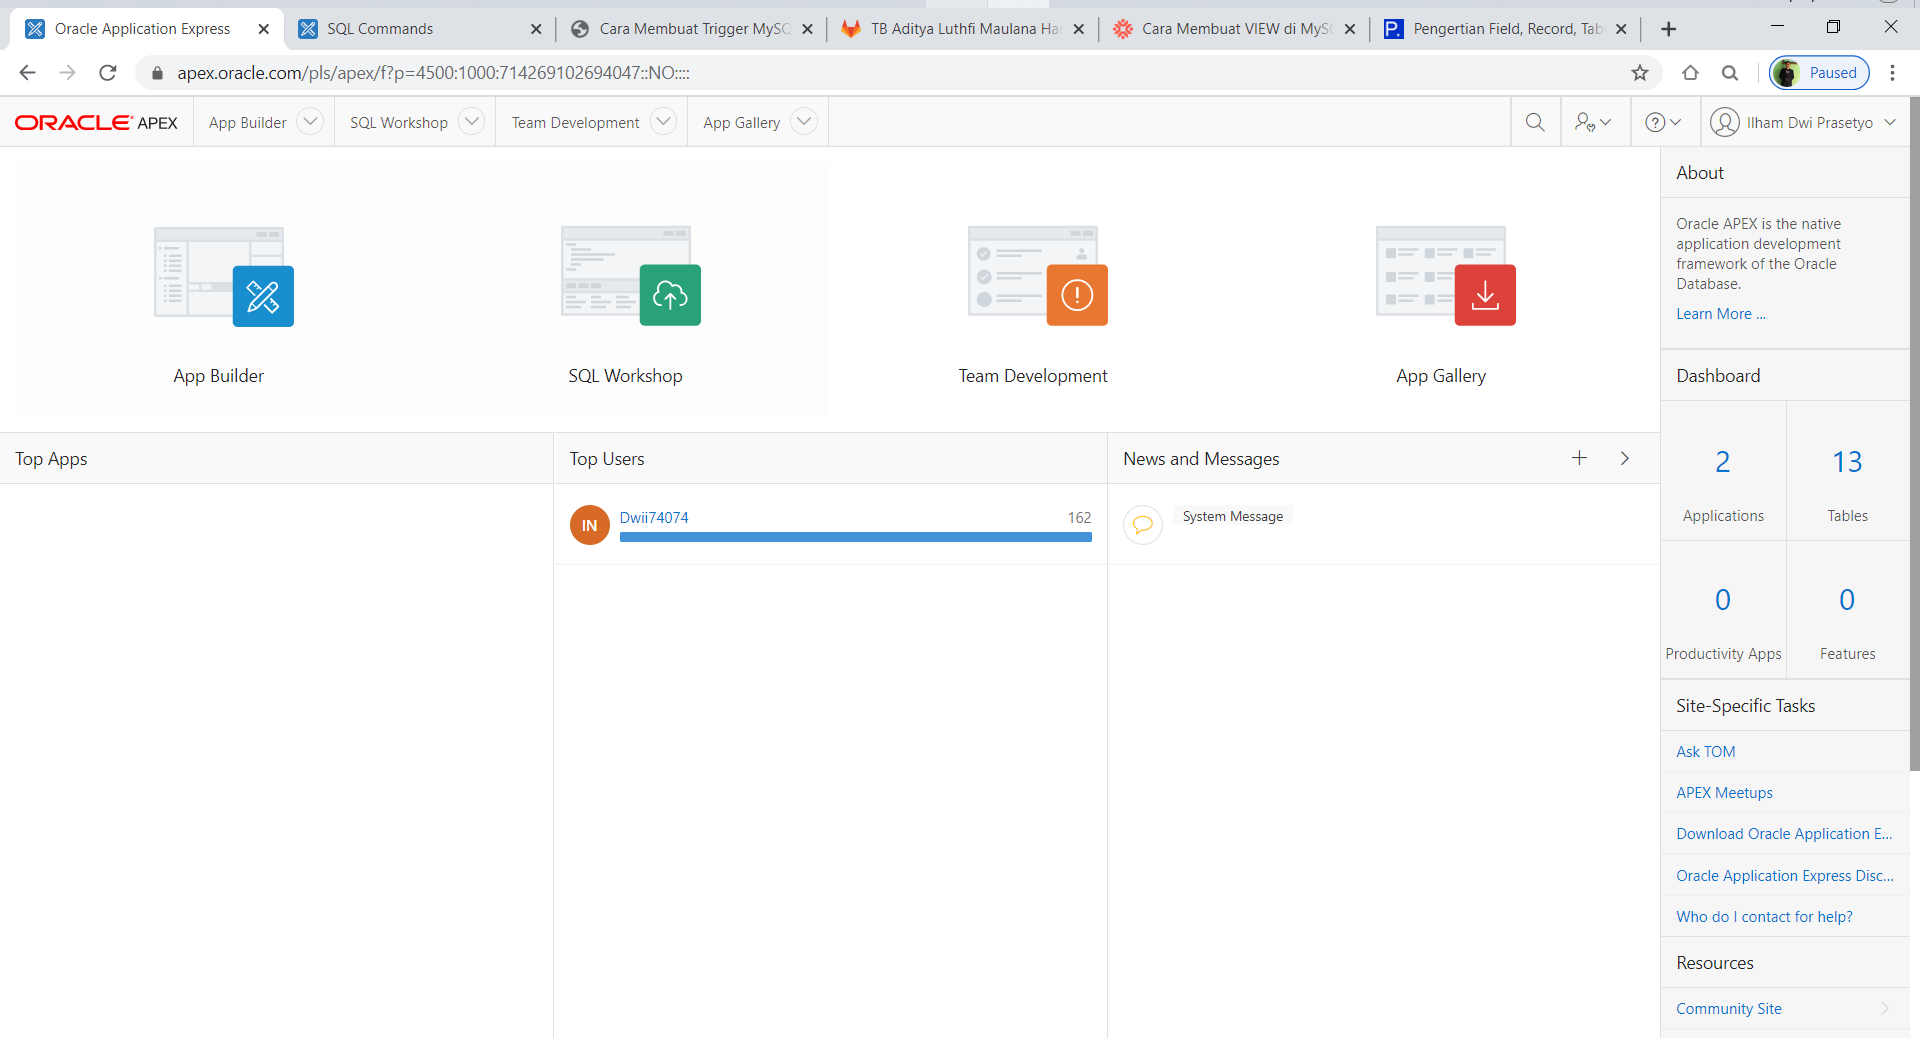
\includegraphics[width=8cm]{image/1.PNG}}
            \end{figure}
    \item Pilih import,jika belum mempunyai data.
    \begin{figure}[h]
            \centerline{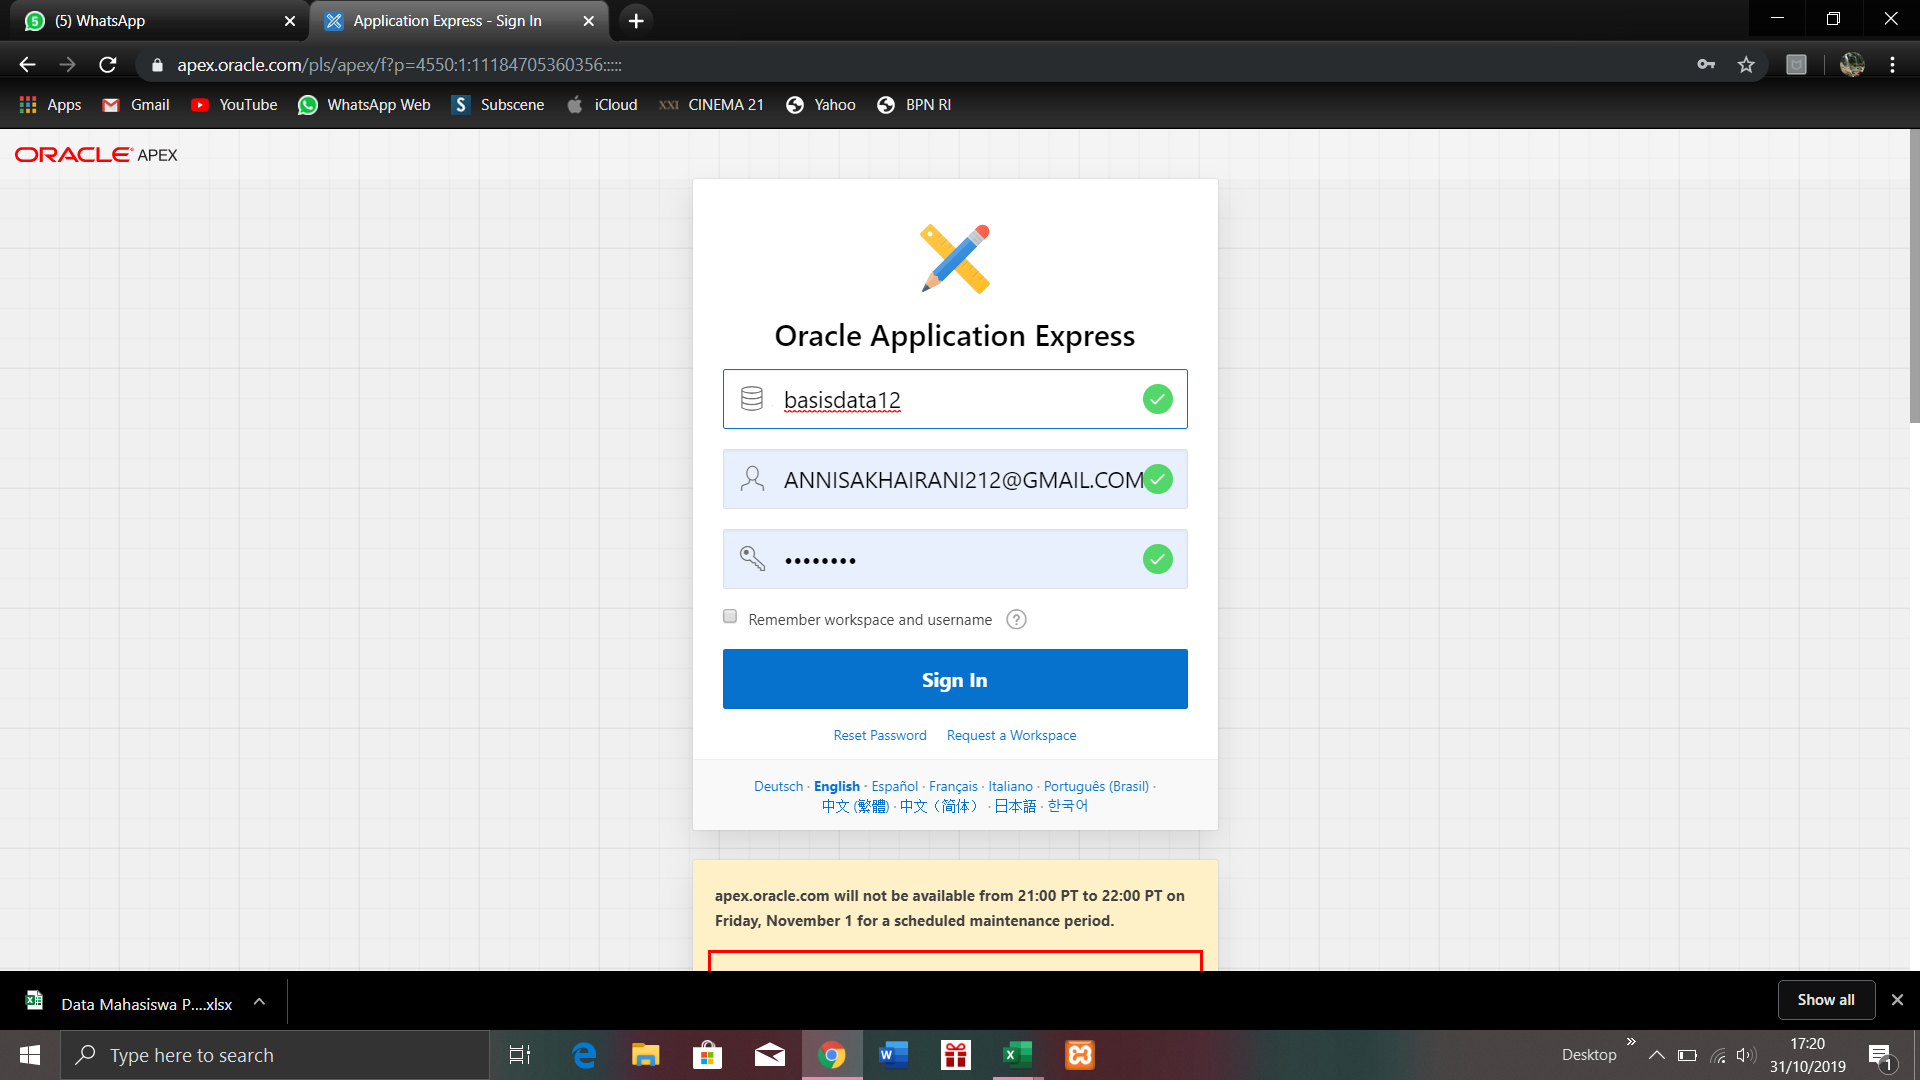
\includegraphics[width=8cm]{image/2.png}}
            \end{figure}
    \newpage\item Choose file lalu next.
    \begin{figure}[h]
            \centerline{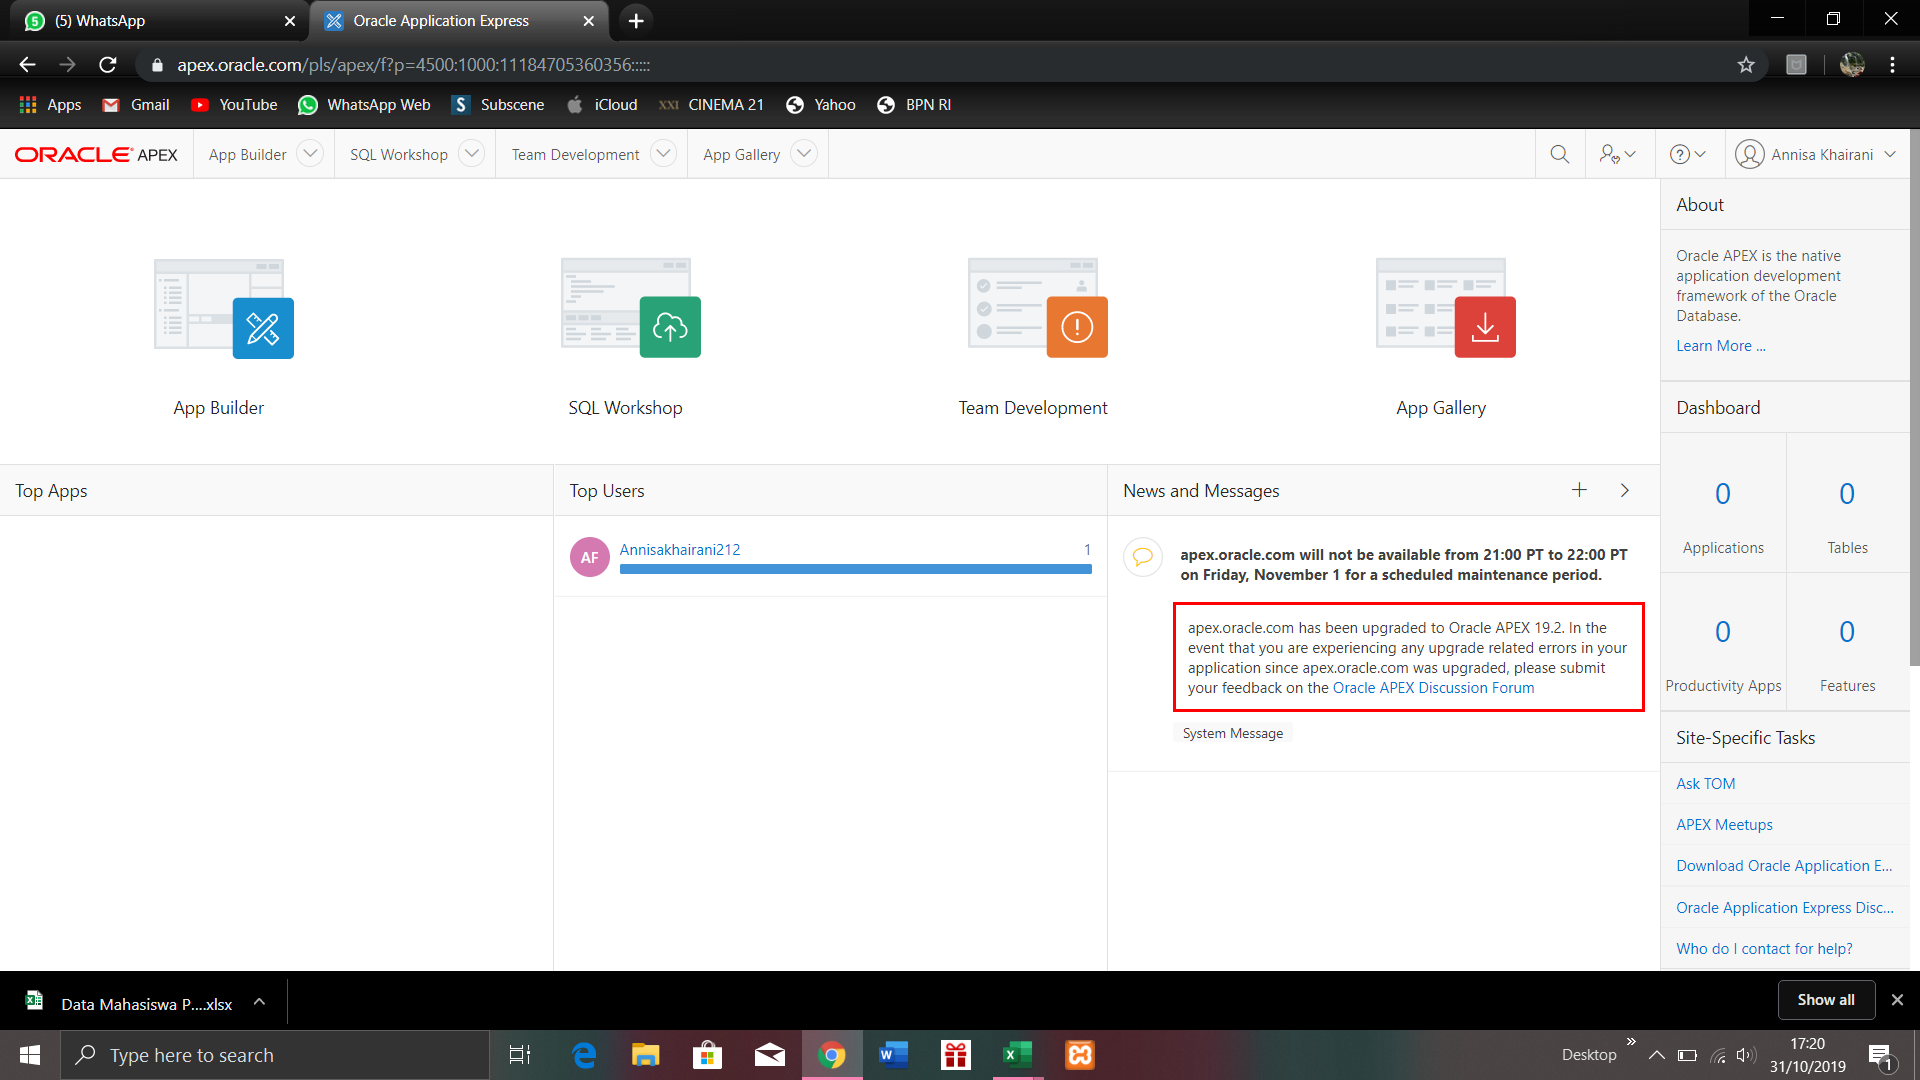
\includegraphics[width=8cm]{image/3.png}}
            \end{figure}
    \item	Lalu akan muncul gambar seperti dibawah. Lalu kita Klik next
    \begin{figure}[h]
            \centerline{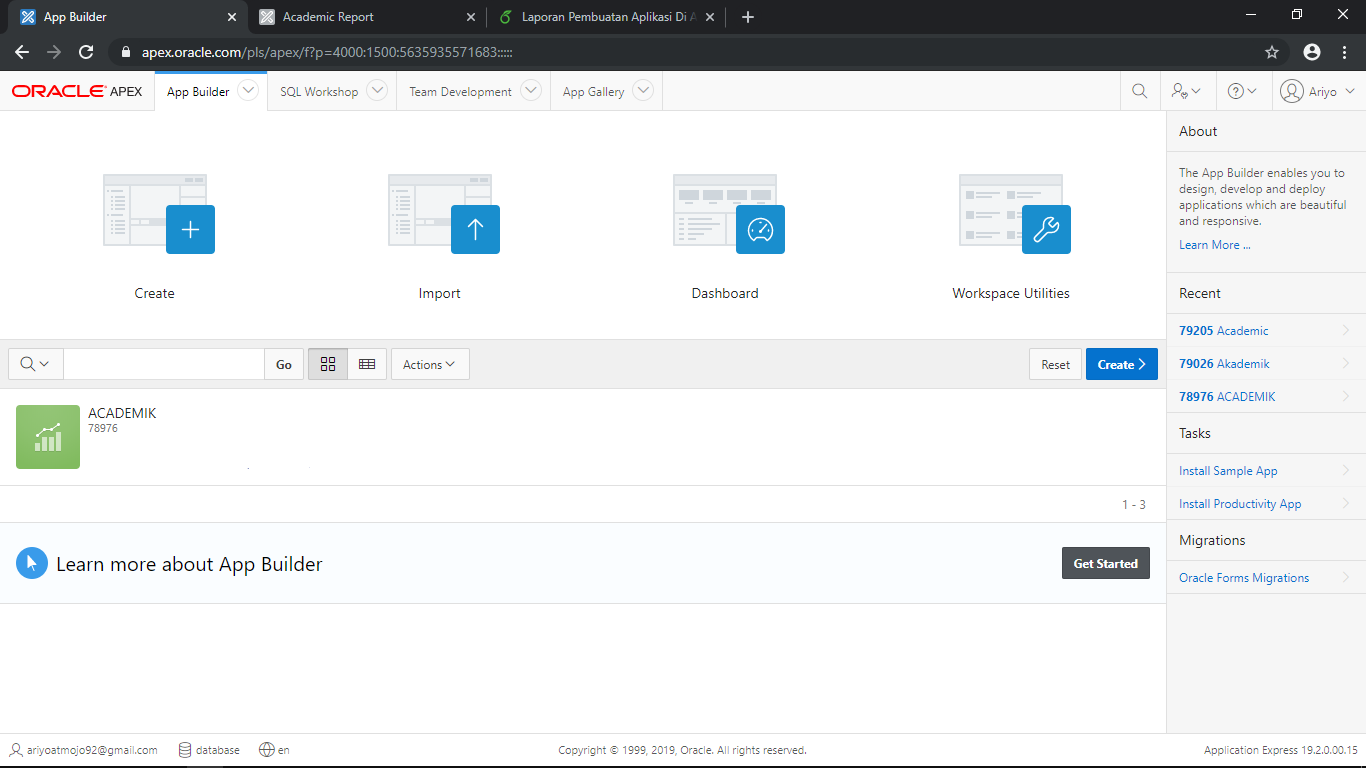
\includegraphics[width=8cm]{image/4.png}}
            \end{figure}
    \item Setelah next, akan muncul seperti ini kemudian kita pilih install application.
    \begin{figure}[h]
            \centerline{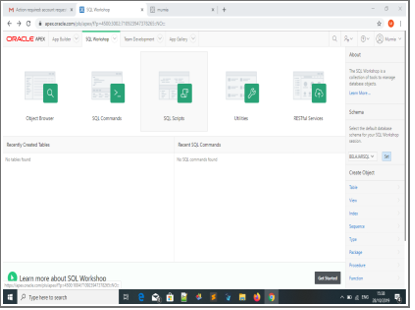
\includegraphics[width=8cm]{image/5.PNG}}
            \end{figure}
    \newpage \item Untuk mengetahui data sudah terinstall atau belum, klik sql Workshop lalu pilih object browser. Jika data muncul berarti telah berhasil
    \begin{figure}[h]
            \centerline{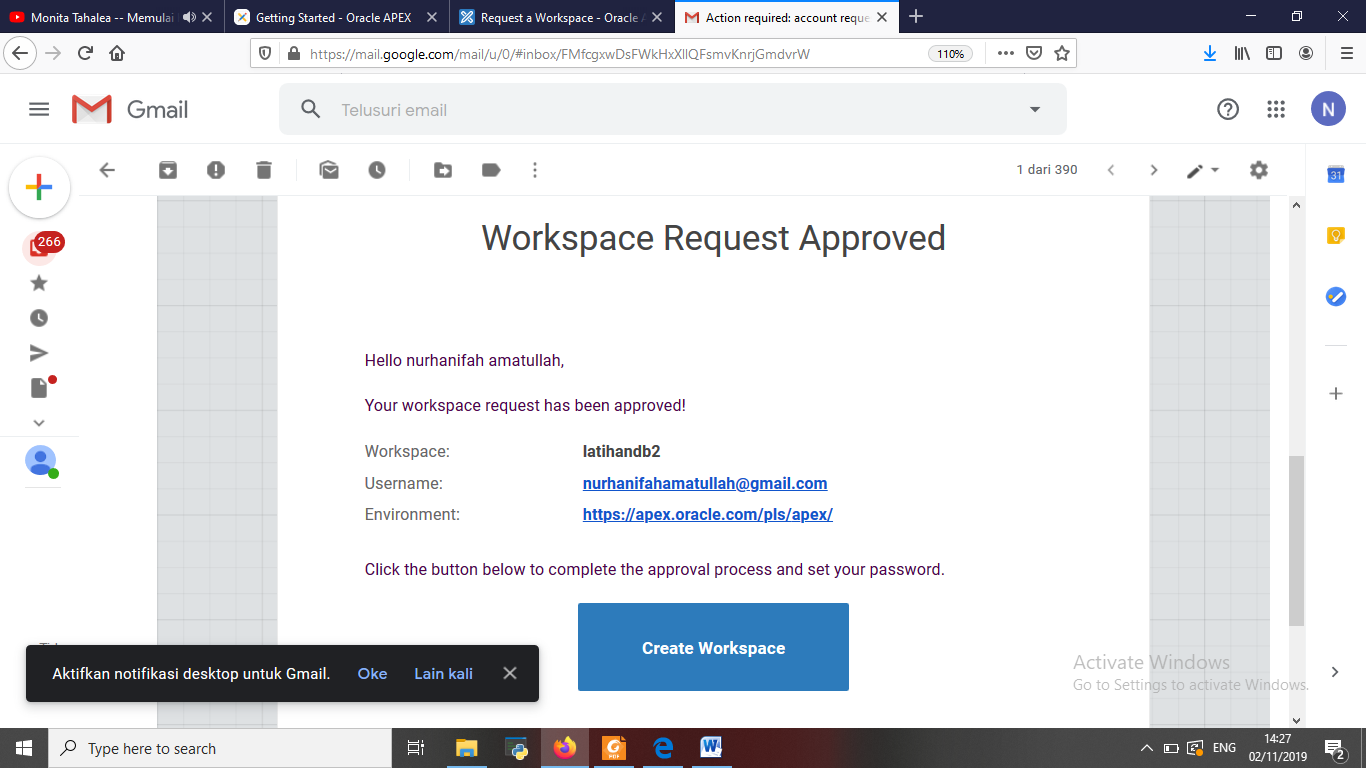
\includegraphics[width=8cm]{image/6.png}}
            \end{figure}
    \newpage \item Lalu kita kembali ke halaman utama, kemudian klik app builder
    \begin{figure}[h]
            \centerline{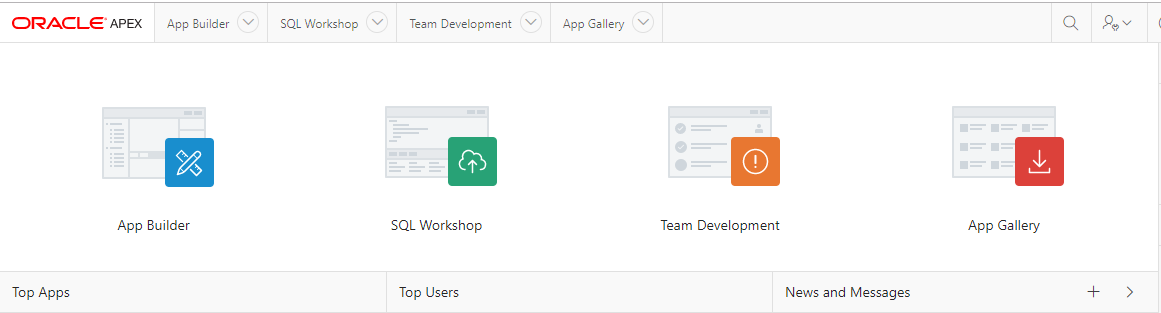
\includegraphics[width=8cm]{image/7,1.png}}
            \end{figure}
    \item Klik Creat a new application
           \begin{figure}[h]
            \centerline{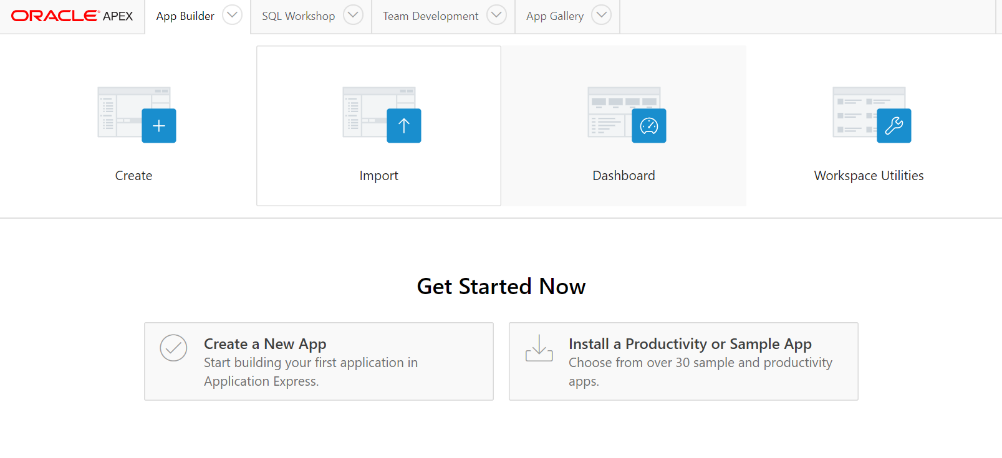
\includegraphics[width=8cm]{image/7,2.png}}
            \end{figure}
    \item 	Klik “from a file”
    \begin{figure}[h]
            \centerline{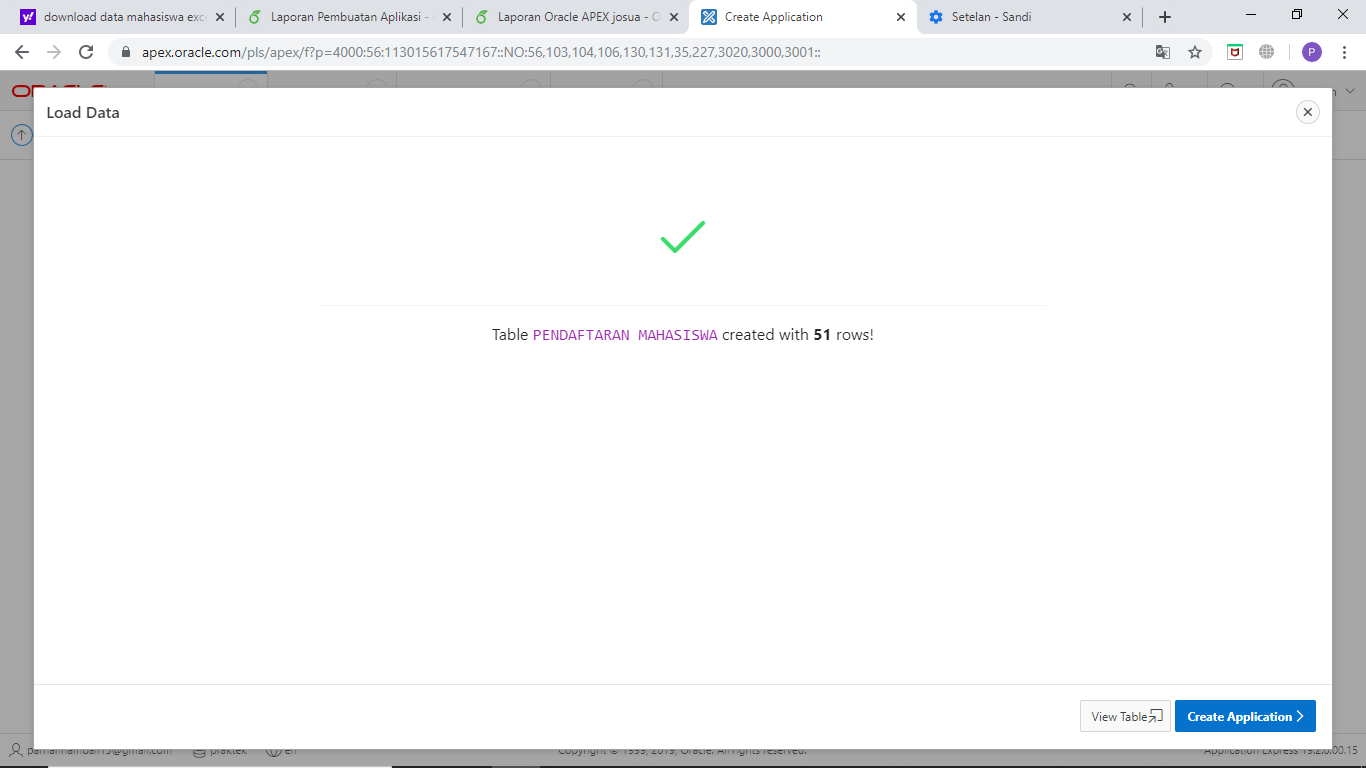
\includegraphics[width=8cm]{image/8.png}}
            \end{figure}
    \item Setelah itu pilih “copy and paste”. Pilih select sample “movie”
    \begin{figure}[h]
            \centerline{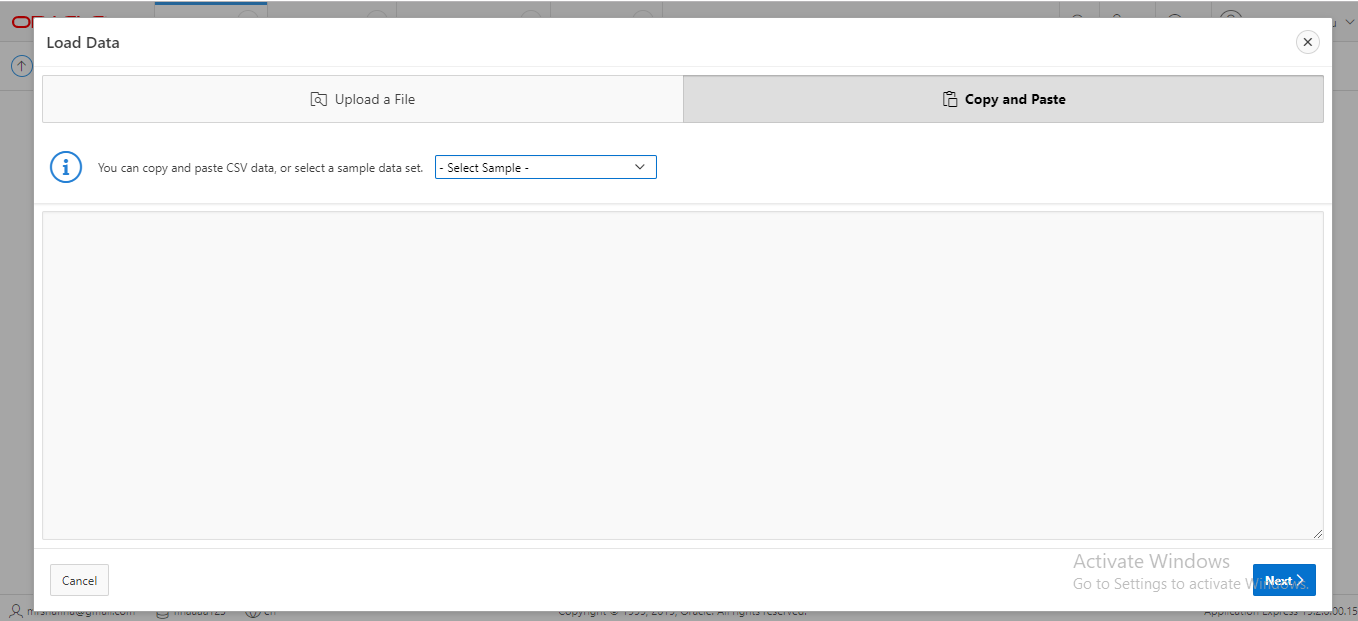
\includegraphics[width=8cm]{image/9.png}}
            \end{figure}
    \newpage \item Setelah muncul seperti gambar dibawah ini, kemudian kita klik next. 
    \begin{figure}[h]
            \centerline{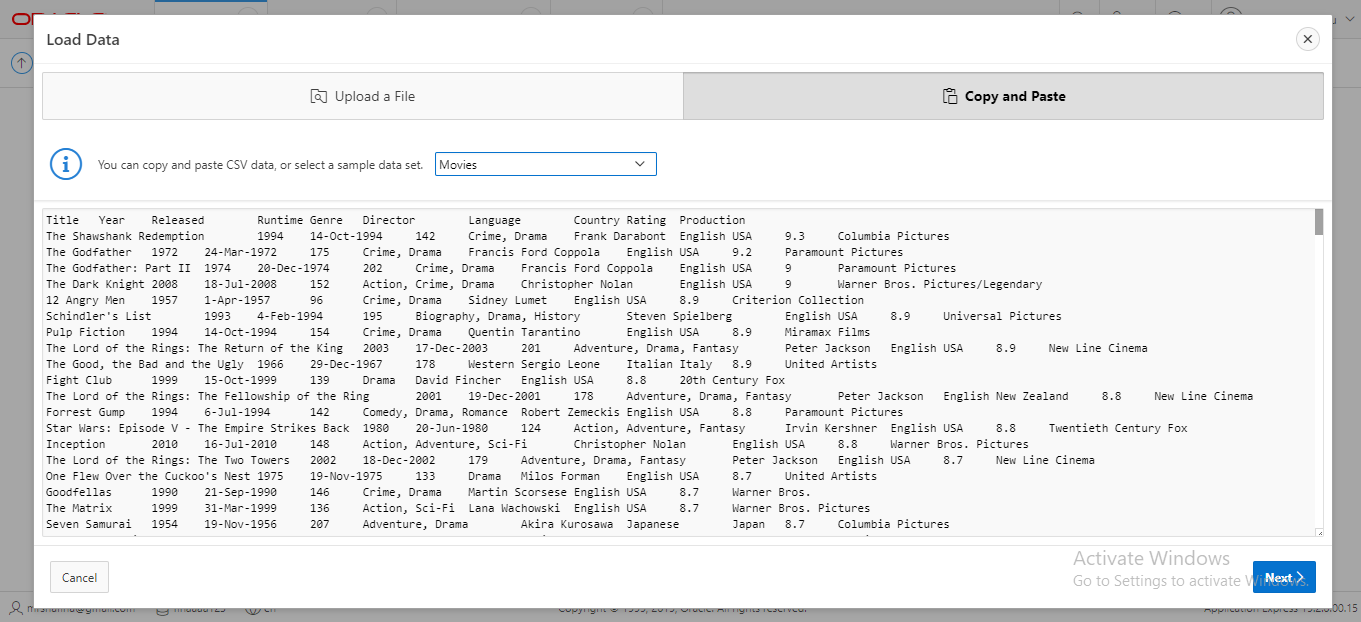
\includegraphics[width=8cm]{image/10.png}}
            \end{figure}
    \item Lalu akan muncul gambar seperti dibawah, lalu isi table nama dengan “MOVIES” dan dengan otomatisnya error table name akan terisi “MOVIES_ERR$” lalu kita klik “Load Data”.
    \begin{figure}[h]
            \centerline{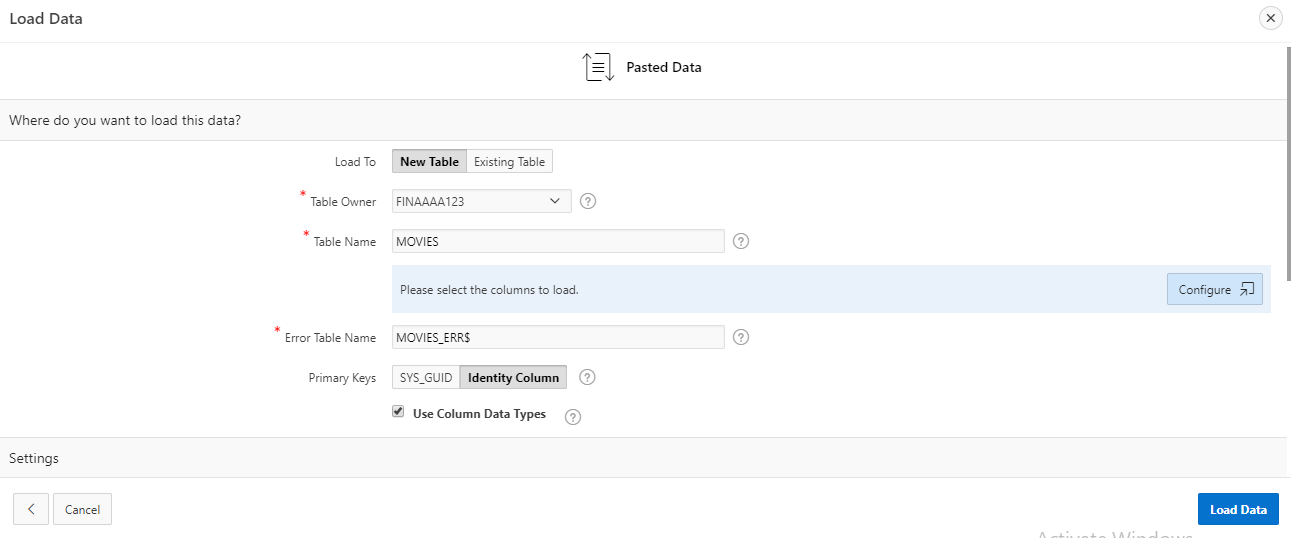
\includegraphics[width=8cm]{image/11.png}}
            \end{figure}
    \item Setelah itu kitamengklik load data, akan muncul seperti gambar dibawah ini (f9).
    \begin{figure}[h]
            \centerline{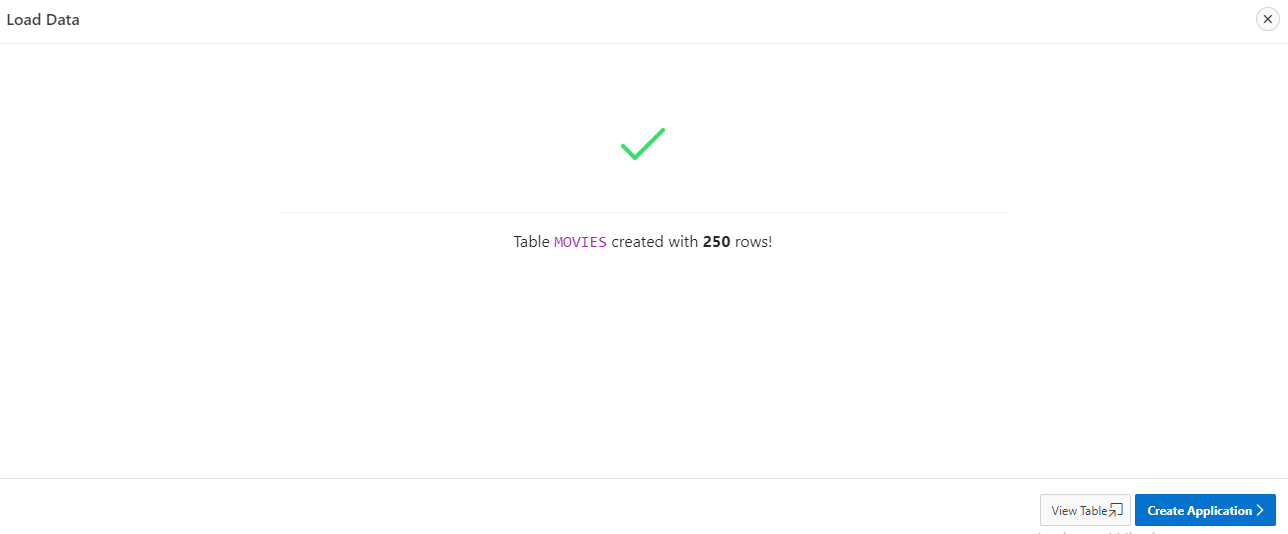
\includegraphics[width=8cm]{image/12.png}}
            \end{figure}
    \newpage \item kemudian kita Klik “create application”. Isi bagian nama dengan “movies app”. Lalu klik tanda panah yang ada di “appearance” akan muncul gambar seperti dibawah ini . appearance sendiri berfungsi untuk mennyetting seperti apa tampilan aplikasi yang akan kita buat. Dari tema, navigasi dan icon untuk aplikasinya
    \begin{figure}[h]
            \centerline{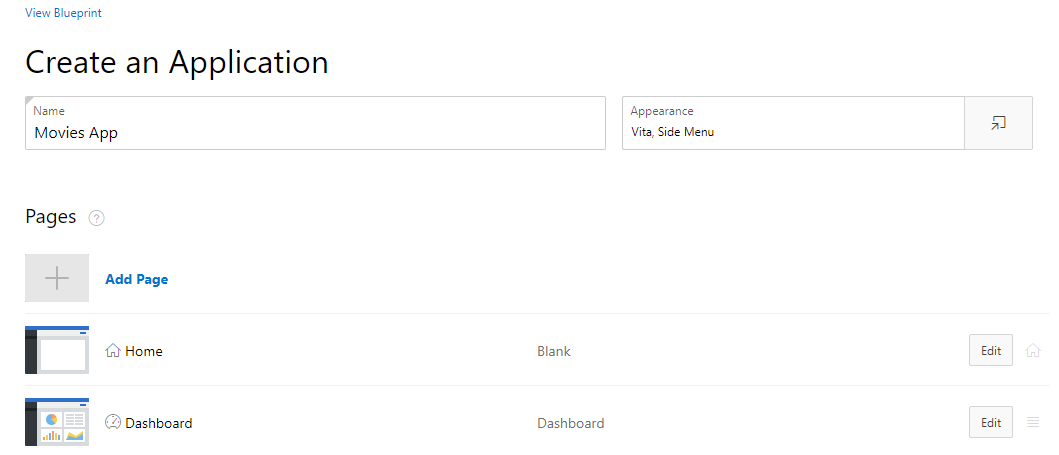
\includegraphics[width=8cm]{image/13.png}}
            \end{figure}
    \item Lalu, kita pilih tema sesuai keinginan kita pada “Theme Style”. Pilih navigasi yang kita inginkan pada ”Navigation”. Dan pilih icon untuk aplikasi pada “application icon”. Setelah sudah dipilih, klik save changes
    \begin{figure}[h]
            \centerline{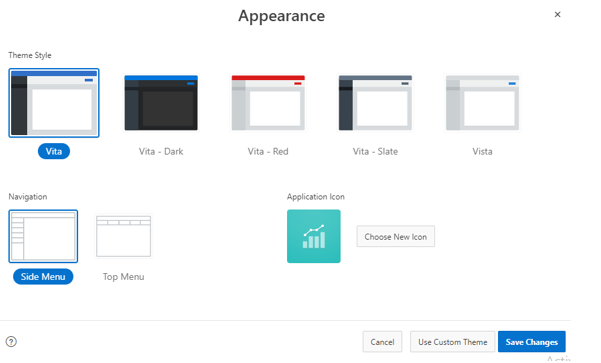
\includegraphics[width=8cm]{image/14.PNG}}
            \end{figure}
    \newpage \item Pada features klik “check all” lalu klik “create application”
    \begin{figure}[h]
            \centerline{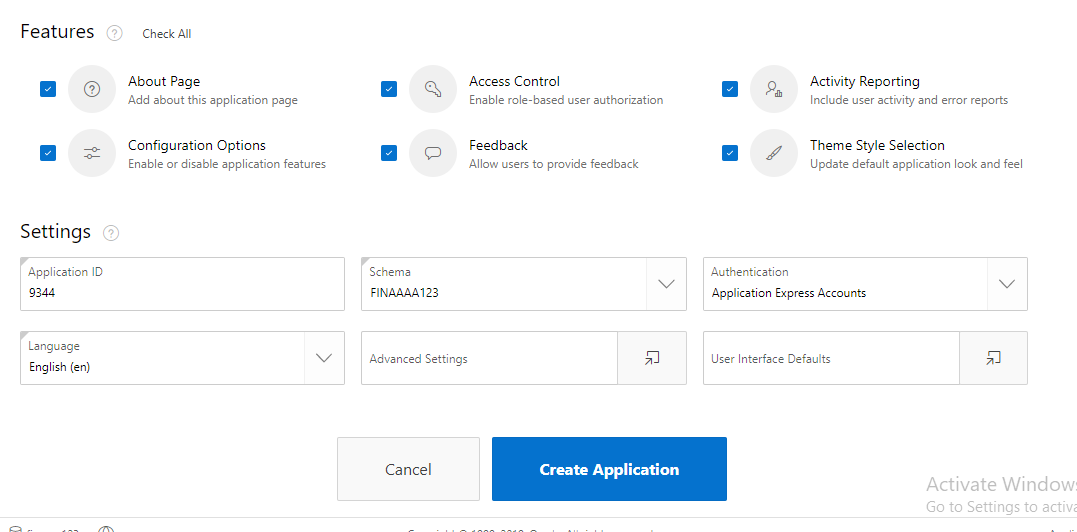
\includegraphics[width=8cm]{image/15.png}}
            \end{figure}
    \item Lalu akan muncul seperti gambar dibawah ini.kemudian kita Klik run application
    \begin{figure}[h]
            \centerline{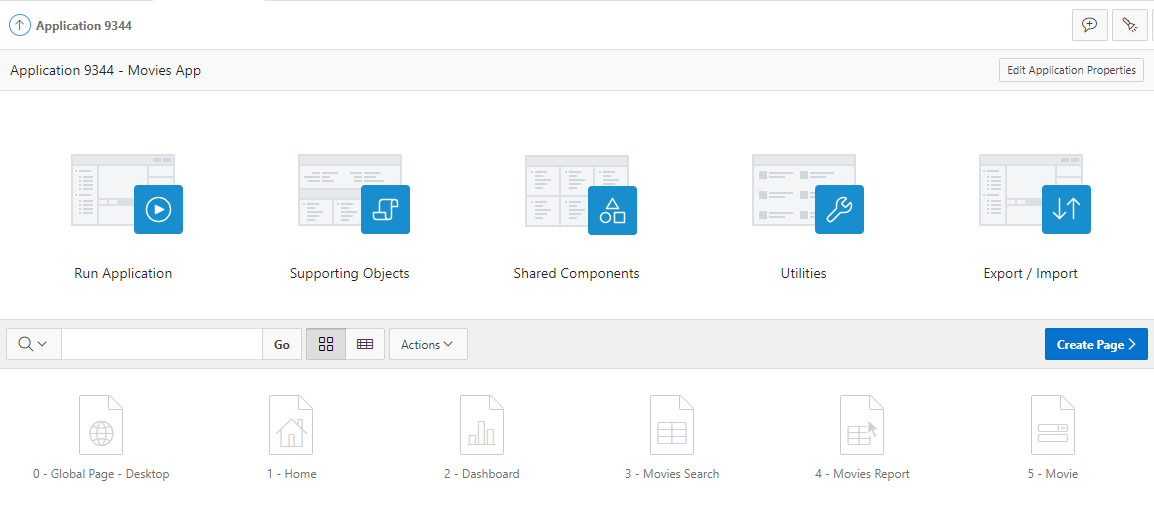
\includegraphics[width=8cm]{image/16.png}}
            \end{figure}
    \item Setelah itu, akan muncul from login untuk masuk ke aplikasi yang kita buat. Lalu sign in 
    \begin{figure}[h]
            \centerline{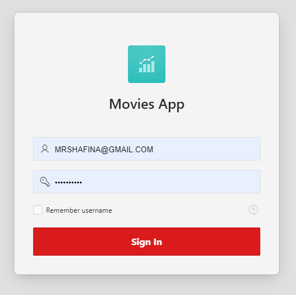
\includegraphics[width=8cm]{image/17.PNG}}
            \end{figure}
   \newpage \item Setelah itu, akan secara langsung masuk pada aplikasi yang kita buat
   \begin{figure}[h]
            \centerline{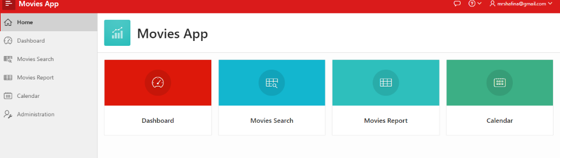
\includegraphics[width=8cm]{image/18.PNG}}
            \end{figure}
\newpage \section{SQL Developer Data Modeler }
\subsection{Oracle SQL Developer Data Modeler menewarkan berbagai kemampuan pemodelan data dan basis data, yang memungkinkan untuk:}
\begin{enumerate}
    \item Menangkap  aturan dan Infoormasi bisnis
    \item Membuat dan memproses Model Logical , Relational, dan Physical
    \item Menyimpan informasi metadata dalam file XML
    \item Menyingkron Model relasional dengan kamus data
\end{enumerate}
\subsection{Konsep Kunci:}
\begin{enumerate}
    \item Buat model logis menggunakan SQL Data 
    \item Modeler Forward Engineer Model Logical ke Relational Model
\end{enumerate}
\subsubsection{Reverse Engineer Model Relational menerapkan standar penamaan menggunakan:}
\begin{enumerate}
    \item Glosarium
    \item Templete penamaan 
\end{enumerate}
\subsection{Mengunduh Oracle SQL Developer Data Modeler}
 \begin{enumerate}
       \item Untuk mengunduh file instalasi, buka oracle technology network di :
http://www.oracle.com.technetwork/developer-tools/datamodeler/download/index.html
        \item Pastikan anda memiliki JRE yang diinstal, jika tidak, untuh dari oracle technology network di:
http://www.oracle.com/technetwork/jave/javase/downloads/index.html
   \end{enumerate}
\subsubsection{Terlebih dahulu kitaBuka Oracle SQL Developer Data Modeler
Setelah file zip Data Modeler diunduh:}
\begin{enumerate}
    \item Ekstrak file zip ke folder apa pun, didalam folder itu perluas folder data modeler
    \item Klik dua kali data modeler.exe untuk 32-bit dan klik dua kali model data 64.exe untuk 64-bit
    \item Referensi informasi berharga di halaman awal (Halaman ini dapat dibuka kembali dengan mengklik Bantuan , Halaman Awal)
    \item Tutup Start Windows
    \item Ready Go
    \item kemudian kita buat entitas ini dalam SQL Data Modeler
\end{enumerate}
\subsection{Kesimpulan}
Oracle SQL Data Modeler memiliki fitur-fitur canggih yang membuat  pembuatan Model Logikal dan Relasional sangat mudah dan intuitif.

\newpage \section{Quick Sql}
\begin{enumerate}
    \item Masuk Ke Oracle, pilih sign in
\begin{figure}[h]
            \centerline{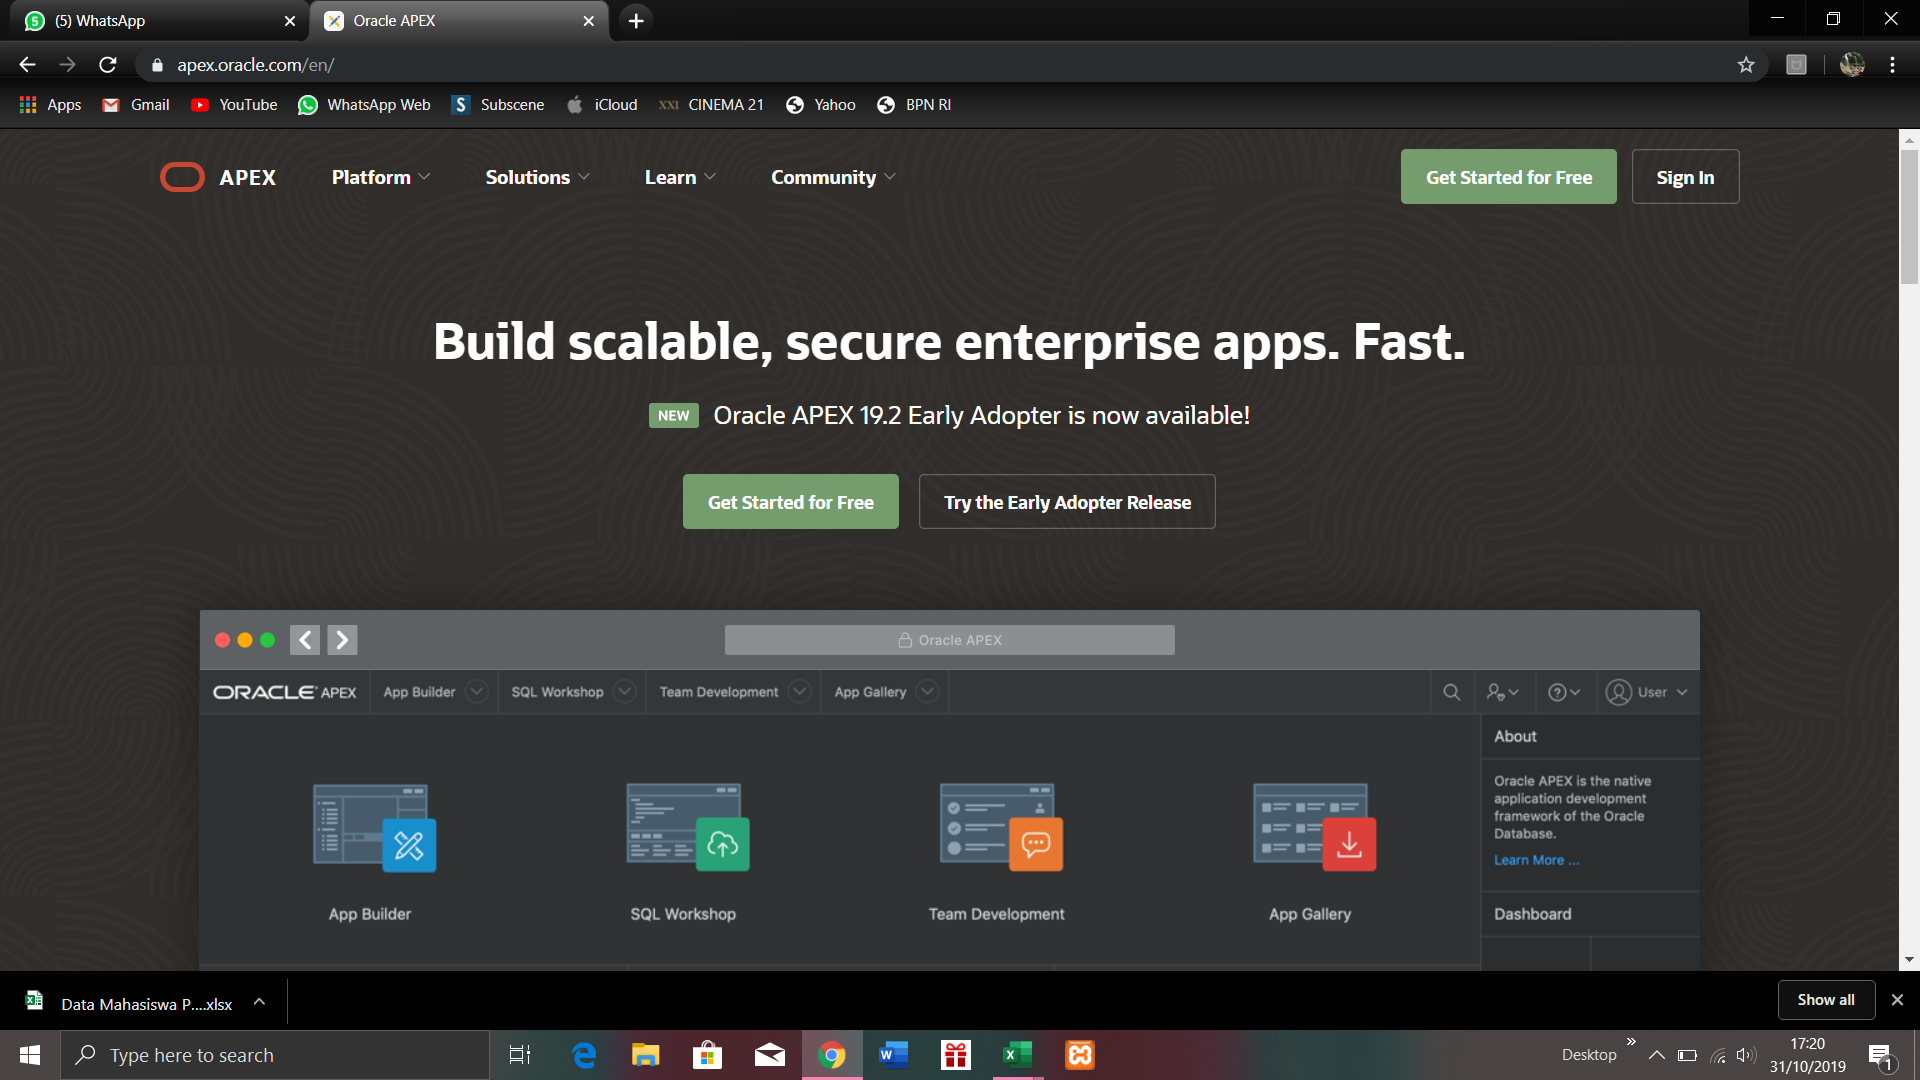
\includegraphics[width=8cm]{image/1.png}}
            \end{figure}
    \item Lalu masukkan workspacae,username,dan password yang kalian punya atau buat aku jika kalian belum mempunyai akun
    \begin{figure}[h]
            \centerline{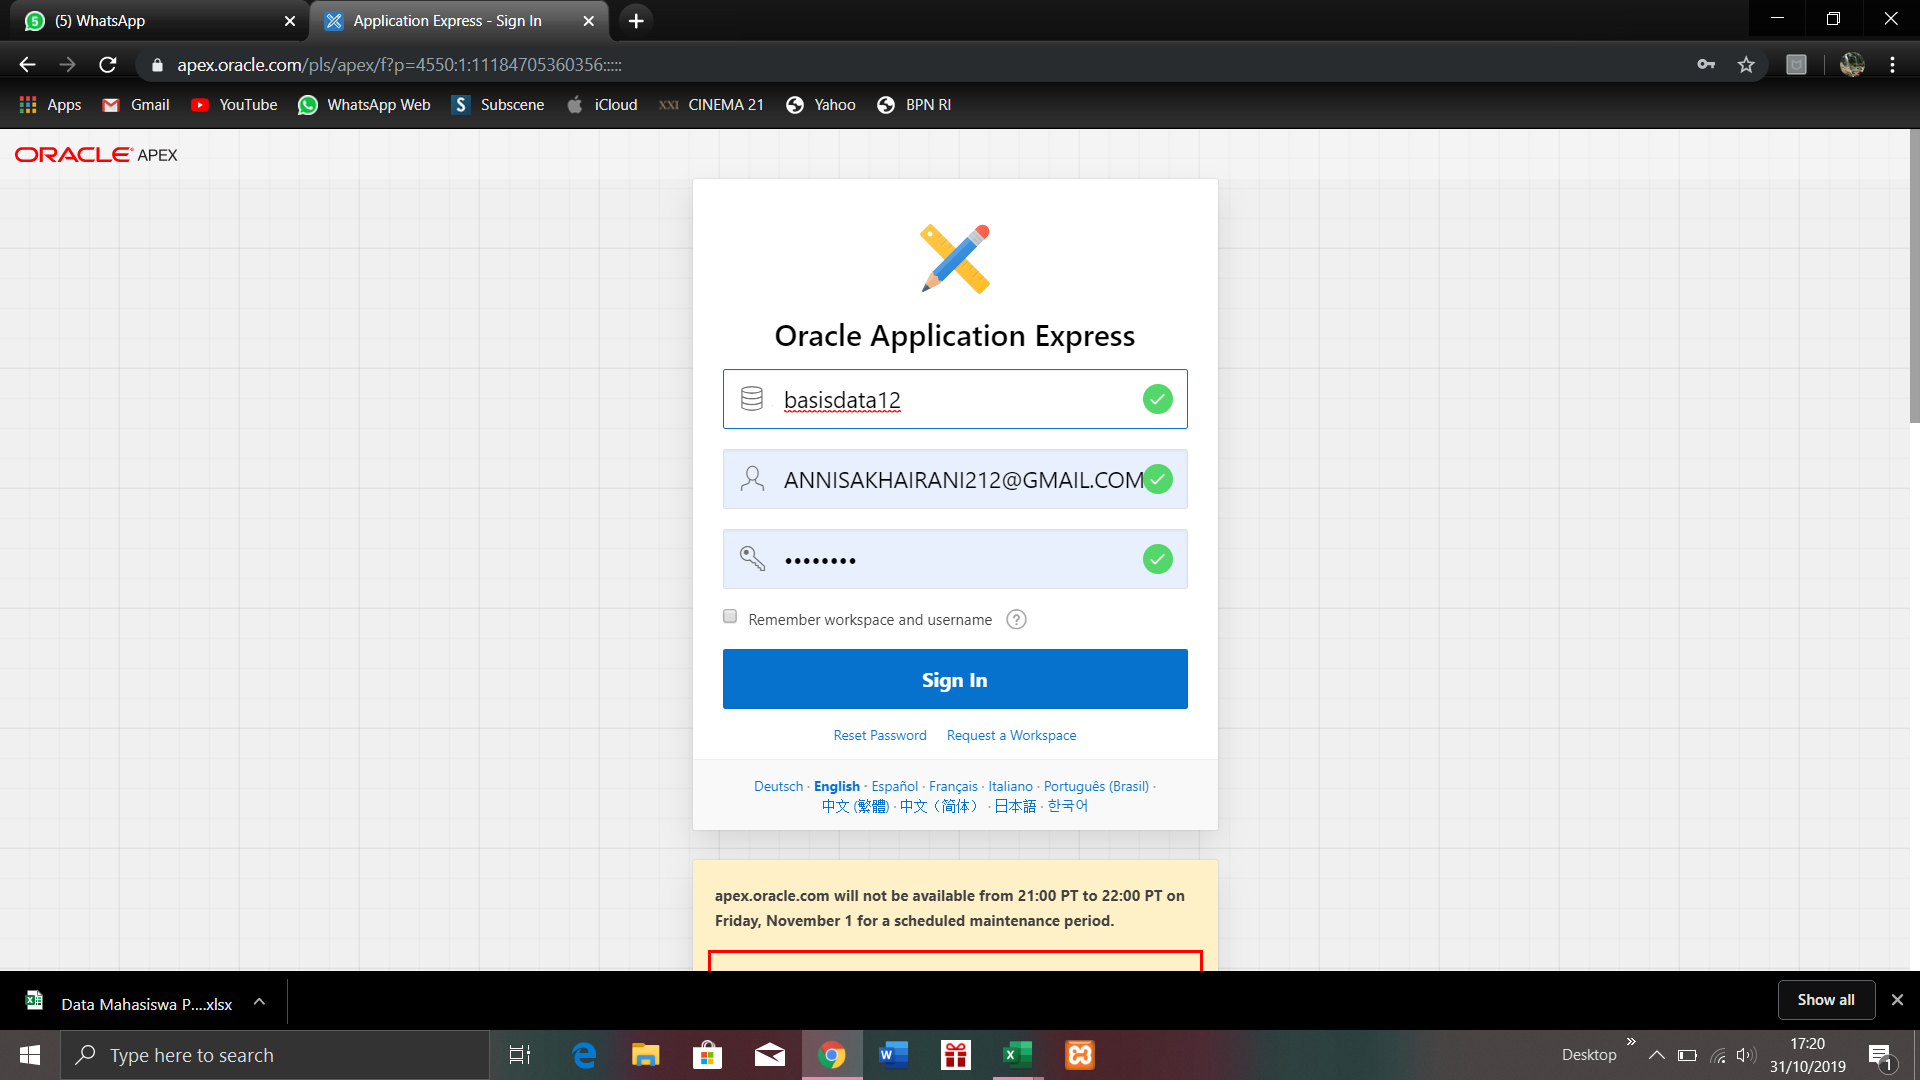
\includegraphics[width=8cm]{image/2.png}}
            \end{figure}
    \newpage \item Setelah itu akan muncul tampilan seperti dibawah ini. Lalu pilih sql workshop dan pilih utilities kemudia pilih quick sql.
    \begin{figure}[h]
            \centerline{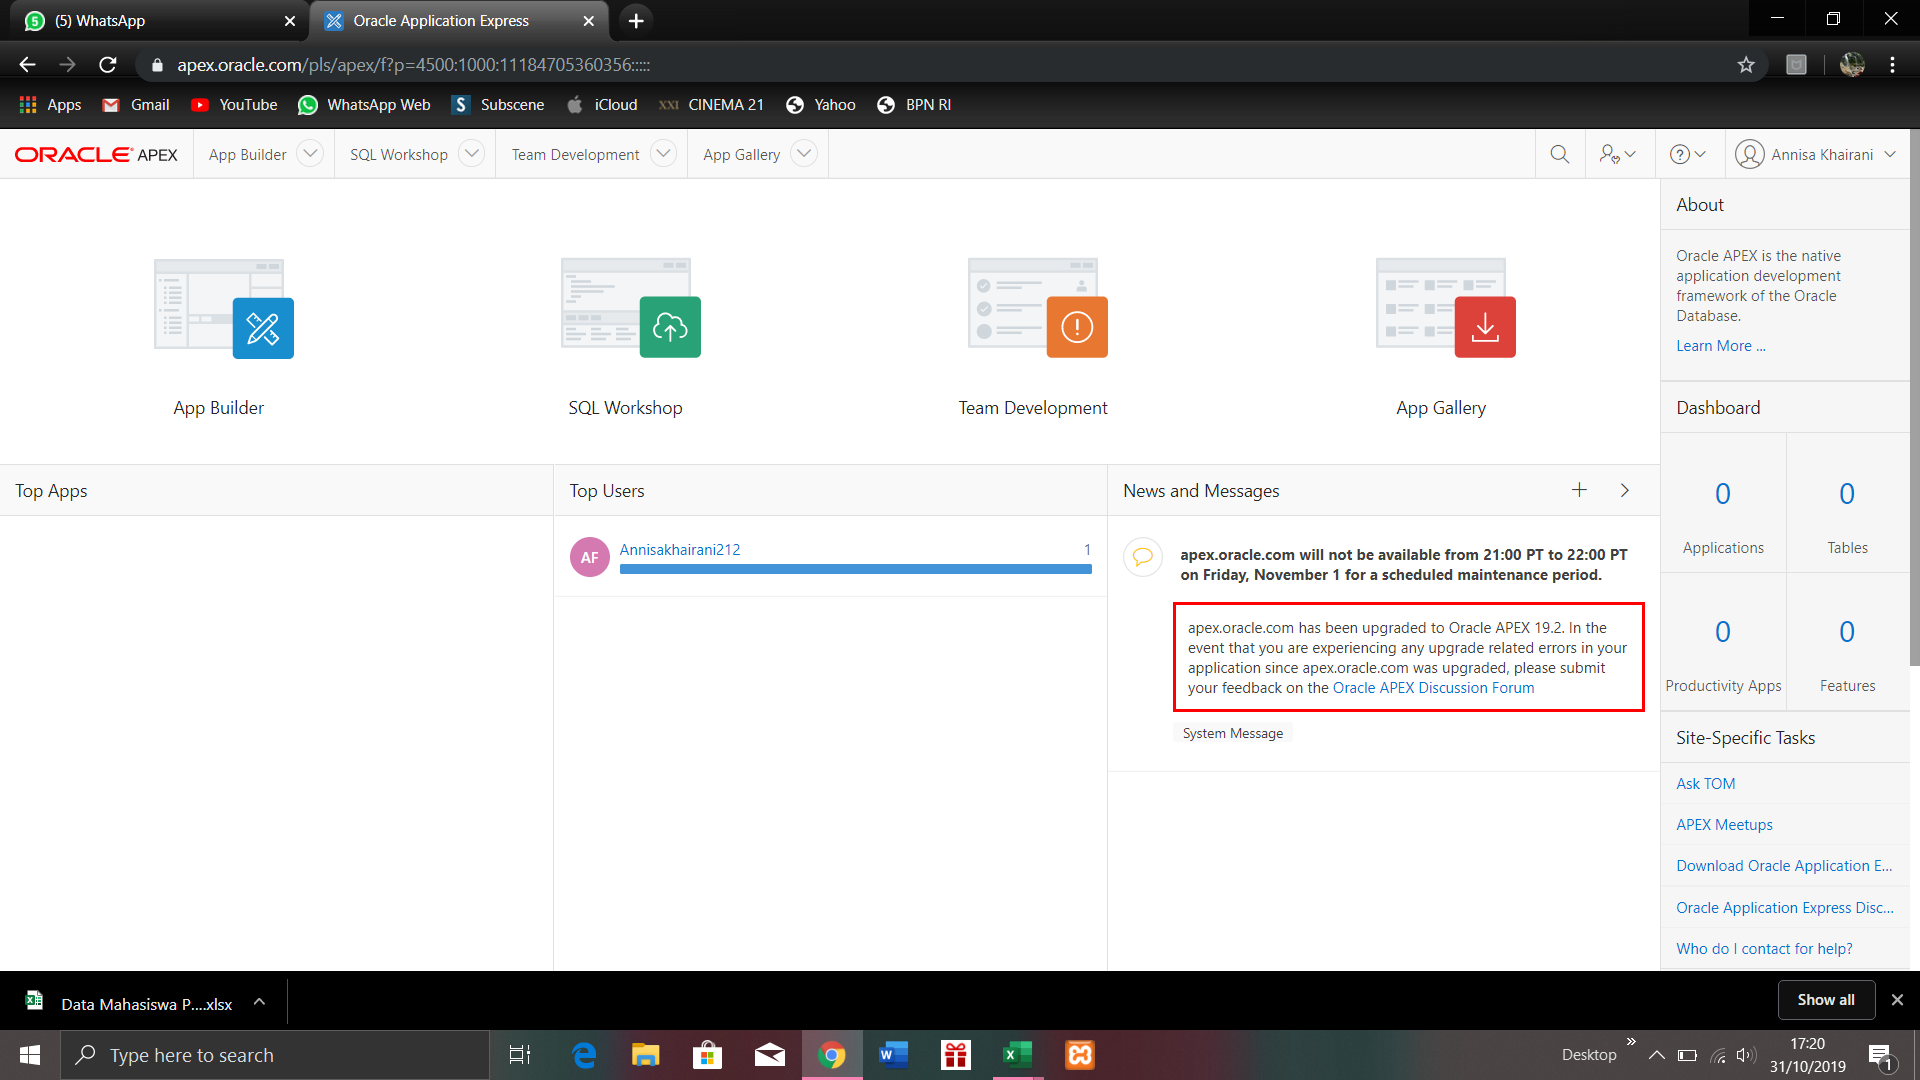
\includegraphics[width=8cm]{image/3.png}}
            \end{figure}
    \item lalu akan muncul tampilan seperti ini.  Maka setelah itu kalian dapat menuliskan kodingan atau program yang akan di jalankan
    \begin{figure}[h]
    \newpage \centerline{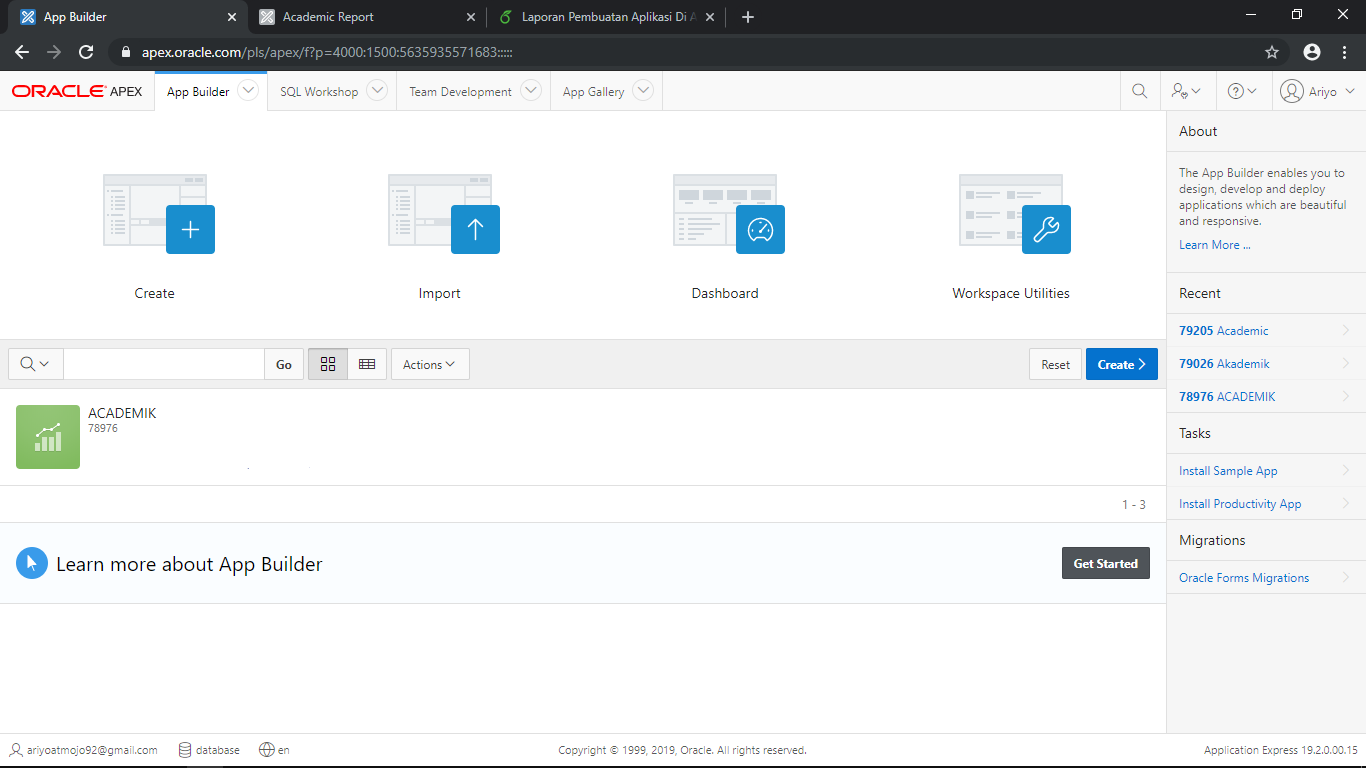
\includegraphics[width=6cm]{image/4.png}}
\end{figure}
    \item  Setelah itu pilih sql workshop
    \begin{figure}[h]
            \centerline{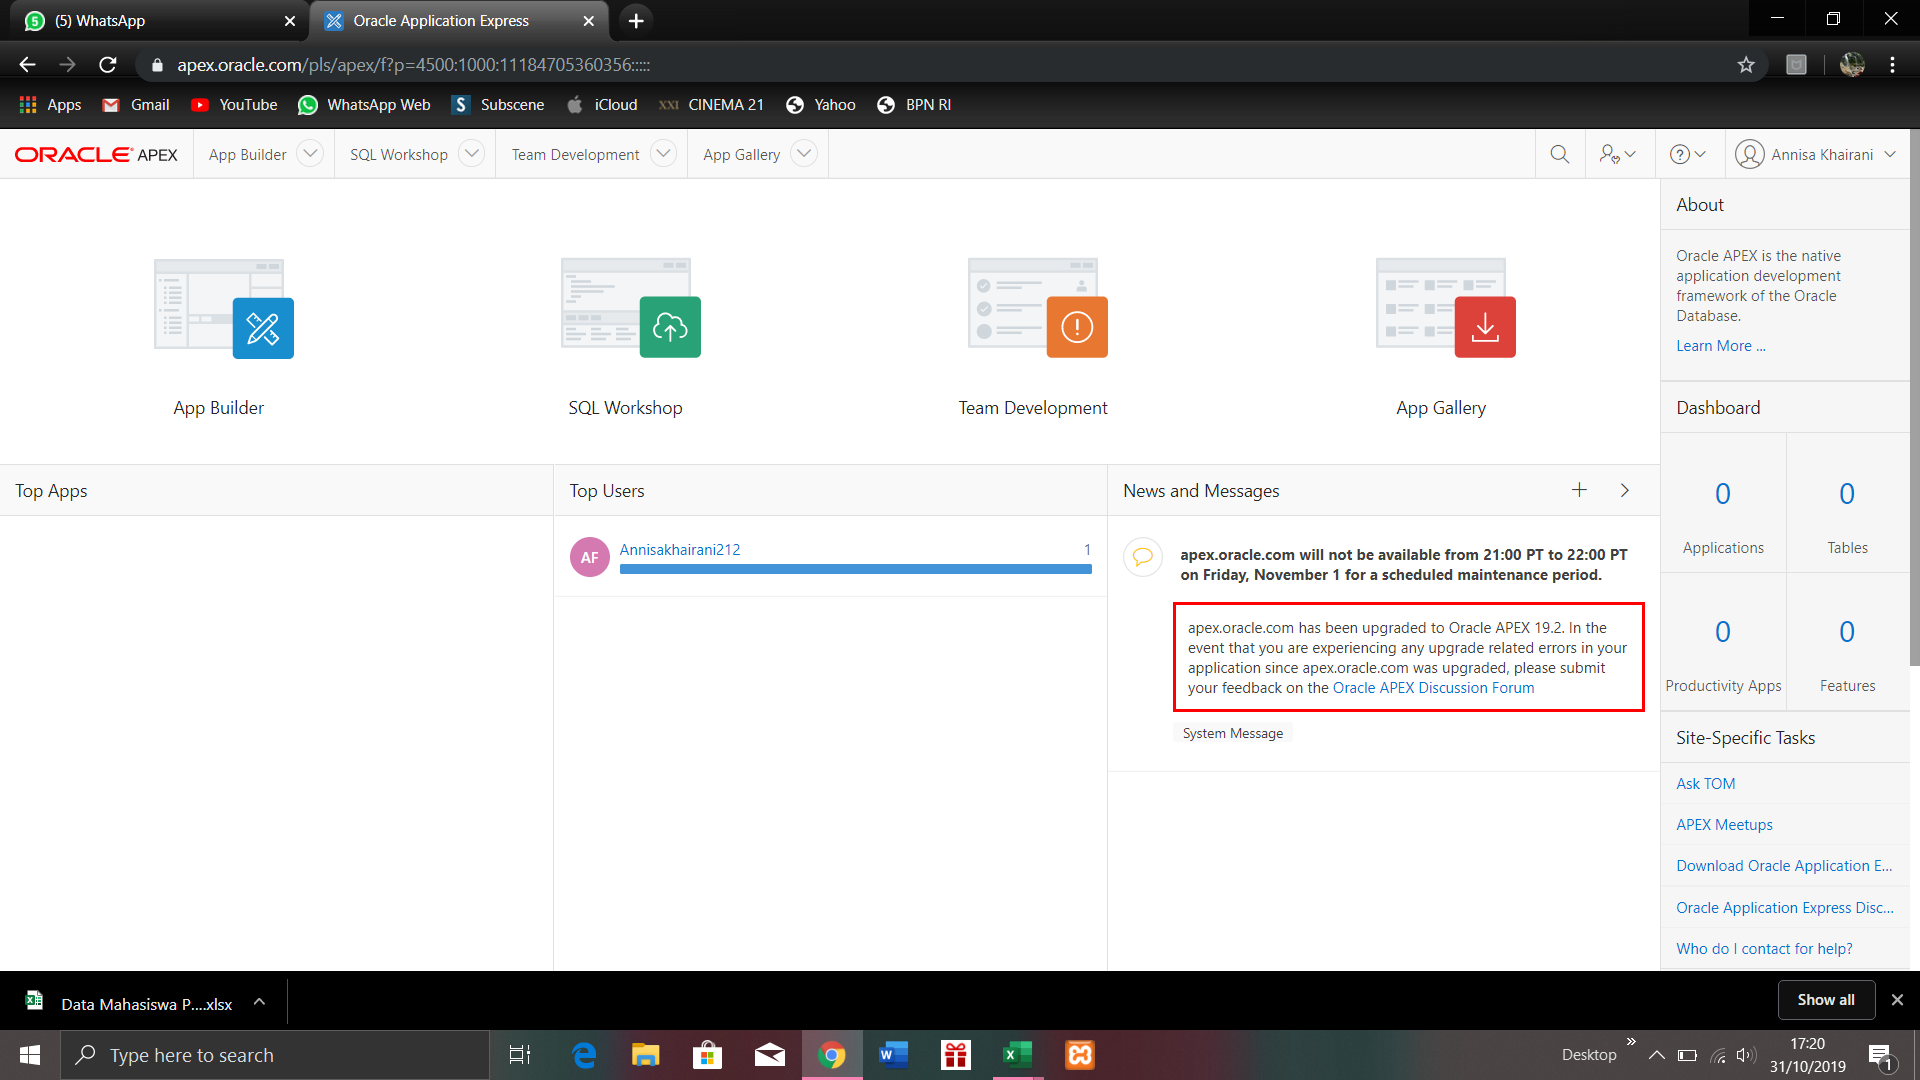
\includegraphics[width=8cm]{image/3.png}}
            \end{figure}
    \newpage \item Setelah itu pilih sql scripts
    \begin{figure}[h]
            \centerline{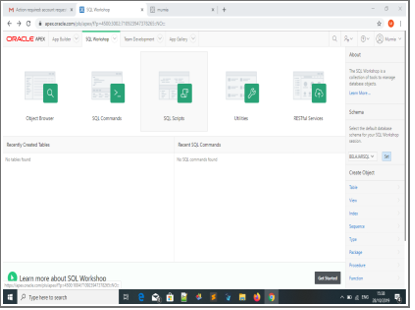
\includegraphics[width=8cm]{image/5.PNG}}
            \end{figure}
    \item Maka kalian akan melihat seperti ini, lalu pindahkan kodingan atau program yang kita tulis di quick sql.
    \begin{figure}[h]
            \centerline{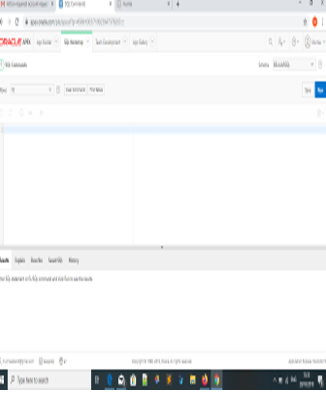
\includegraphics[width=8cm]{image/6.PNG}}
            \end{figure}
    \newpage \item Setelah itu kita pilih run script
    \begin{figure}[h]
            \centerline{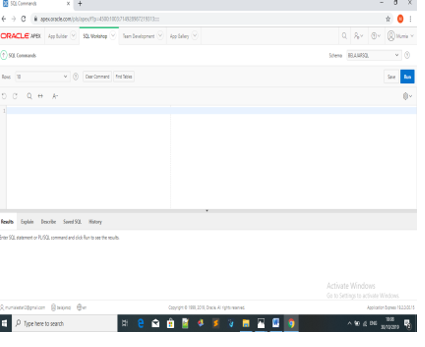
\includegraphics[width=8cm]{image/7.PNG}}
            \end{figure}
    \newpage \item Setelah itu pilih sql command untuk memanggil kodingan atau program yang kita buat
    \begin{figure}[h]
            \centerline{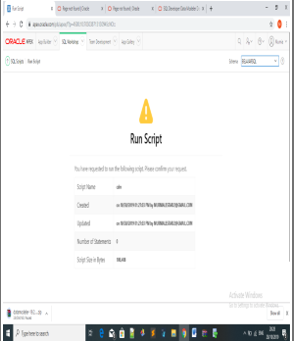
\includegraphics[width=6cm]{image/8.PNG}}
            \end{figure}
\newpage \section{Aplikasi development}
\begin{enumerate}
    \item Buka ilearning.oracle
    \begin{figure}[h]
            \centerline{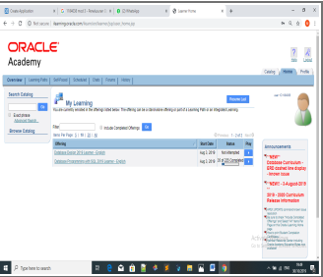
\includegraphics[width=8cm]{image/a.PNG}}
            \end{figure}
    \item Lalu download modul yang kalian mau pada ilearning.
    \item Lalu masuk ke oracleapex.com
    \begin{figure}[h]
            \centerline{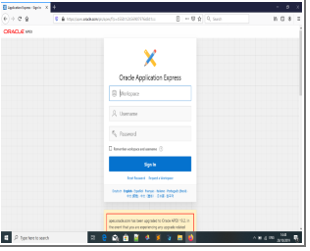
\includegraphics[width=8cm]{image/b.PNG}}
            \end{figure}
    \newpage \item Lalu akan keluar tampilan awal pada oracle apex
    \begin{figure}[h]
            \centerline{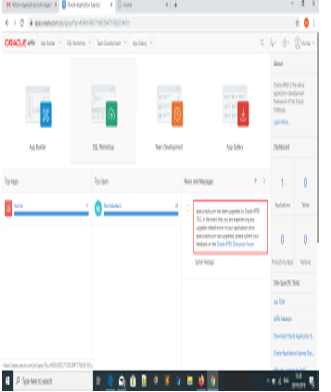
\includegraphics[width=8cm]{image/c.PNG}}
            \end{figure}
    \newpage \item Kemudian kita pilih sql workshop
    \begin{figure}[h]
            \centerline{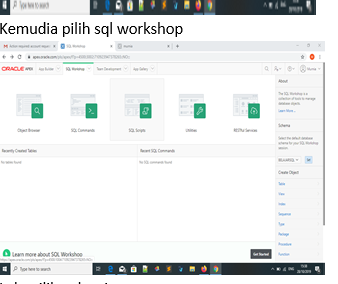
\includegraphics[width=8cm]{image/d.PNG}}
            \end{figure}
    \newpage \item Lalu pilih sql script
    \begin{figure}[h]
            \centerline{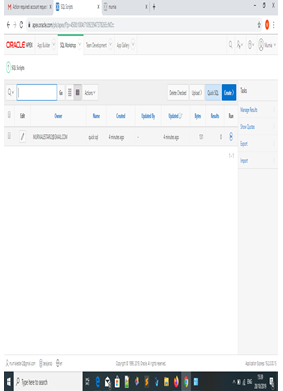
\includegraphics[width=8cm]{image/e.PNG}}
            \end{figure}
    \item Lalu pilih upload script, maka pilih lah file yang akan dimasukkan ke dalam sql script . kemudia akan muncul file yang telah dimasukkan
    \item Lalu tekan tombol run
    \item Setelah itu pergi ke tampilan awal dan pilih aplikasi builder,lalu pilih desktop
    \begin{figure}[h]
            \centerline{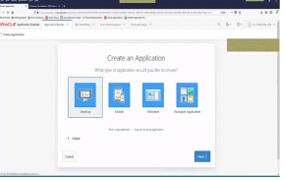
\includegraphics[width=5cm]{image/f.PNG}}
            \end{figure}
    \newpage \item Kemudian kita isi
\newpage \section{CREATE A SIMPLE DATABASE}
\begin{enumerate}
    \item Create Aplikasi baru , jangan lupa Menganti nama menjadi Employe Database Aplication , kemudia Next
    \begin{figure}[h]
          \newpage  \centerline{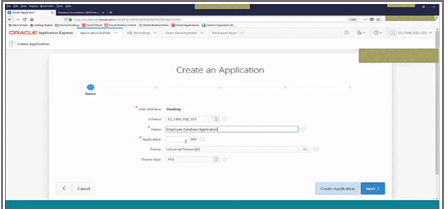
\includegraphics[width=8cm]{image/g.PNG}}
            \end{figure}
    \item Kemudian setelah halaman telah berpindah , akan tampak seperti dibawah ini, kemudian table akan muncul dan klik next
    \begin{figure}[h]
            \centerline{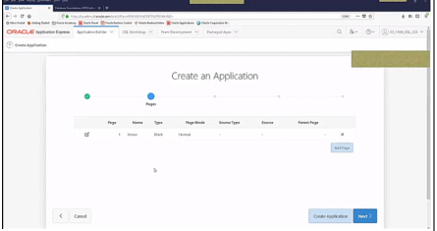
\includegraphics[width=8cm]{image/h.PNG}}
            \end{figure}
    \newpage \item kemudian akan muncul seperti dibawah ini, dan pilih report dan add page kemudian  klik next
\begin{figure}[h]
            \centerline{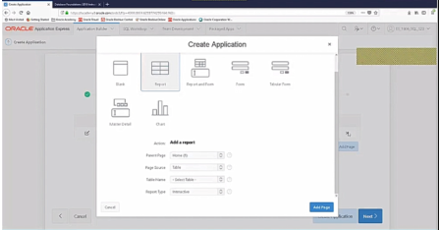
\includegraphics[width=8cm]{image/i.PNG}}
            \end{figure}
    \item Kemudian pilih NO dan klik Next
    \begin{figure}[h]
    \centerline{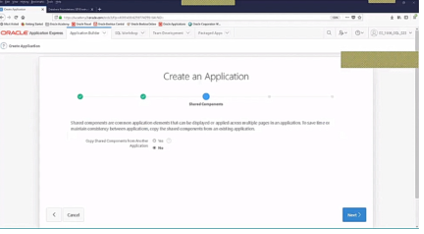
\includegraphics[width=8cm]{image/j.PNG}}
            \end{figure}
    \item Kemudian pada bagian ini ganti application schema menjadi No Autentication, kemudian next
    \begin{figure}[h]
        \newpage\centerline{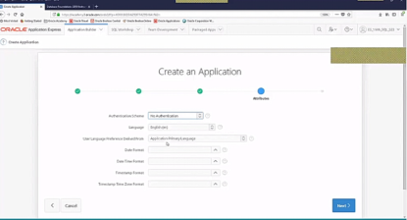
\includegraphics[width=8cm]{image/k.PNG}}
    \end{figure}
    \newpage \item Karena  table sudah  dibuat, klik create application
    \begin{figure}[h]
        \newpage\centerline{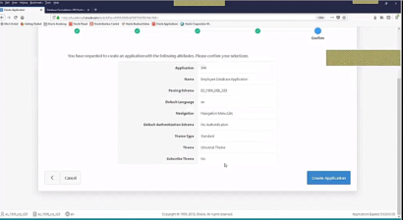
\includegraphics[width=8cm]{image/l.PNG}}
    \end{figure}
    \item Akan muncul kalimat Aplication create successfully maka sudah berhasil membuat aplikasi table nya dulu.jangan lupa untuk view Schema agar bisa liat apa yang telah kita buat
    \begin{figure}[h]
        \centerline{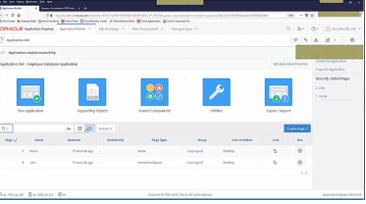
\includegraphics[width=8cm]{image/m.PNG}}
    \end{figure}
    \newpage \item Setelah itu kita run apss kemudian klik job, dan review
    \begin{figure}[h]
        \centerline{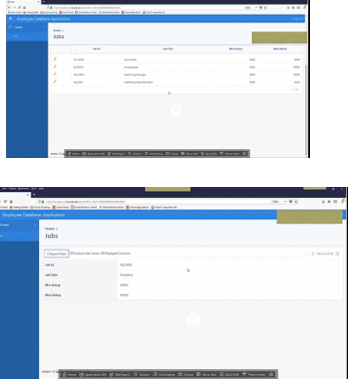
\includegraphics[width=8cm]{image/n.PNG}}
    \end{figure}
    \newpage \item Kemudia balik lagi ke menu sebelumnya untuk dirun aplikasinya
    \begin{figure}[h]
        \centerline{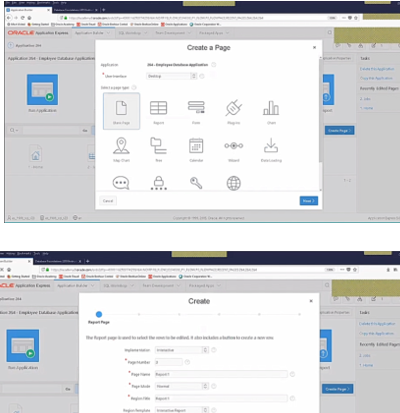
\includegraphics[width=8cm]{image/o.PNG}}
    \end{figure}
    \item Setelah di create  kemudian kita tekan next
    \begin{figure}[h]
        \centerline{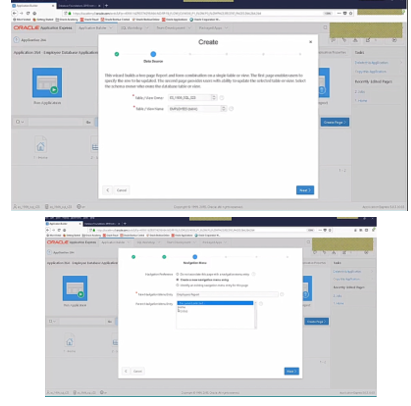
\includegraphics[width=8cm]{image/p.PNG}}
    \end{figure}
    \newpage \item Kemudian pada step berukikutnya pilih icon pencil, kemudian lanjutkan pada step berikutnya
    \begin{figure}[h]
        \centerline{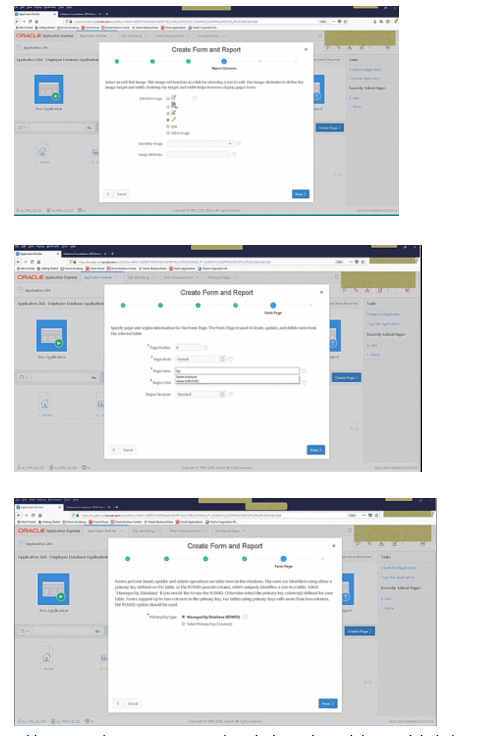
\includegraphics[width=8cm]{image/q.PNG}}
    \end{figure}
    \item Jangan lupa memilih primary key agar mencegah redudansi dan tidak terjadi kekeliruan kemudian next
    \begin{figure}[h]
        \centerline{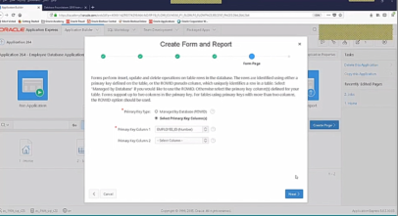
\includegraphics[width=8cm]{image/r.PNG}}
    \end{figure}
    \newpage \item Kemudian kita tekan next sebab data yang diinginkan telah di bentukpada kolom disebelahnya
     \begin{figure}[h]
        \centerline{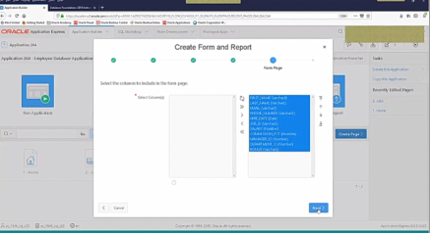
\includegraphics[width=8cm]{image/s.PNG}}
    \end{figure}
    \newpage \item Pembuatan dash board ,seperti biasa membuak dashboard kemudia buka uplication yang telha dibuat, salah satunya adalah yang untuk mengupdate nya kemudian langsung buka agar bisa mengoding
    \begin{figure}[h]
        \centerline{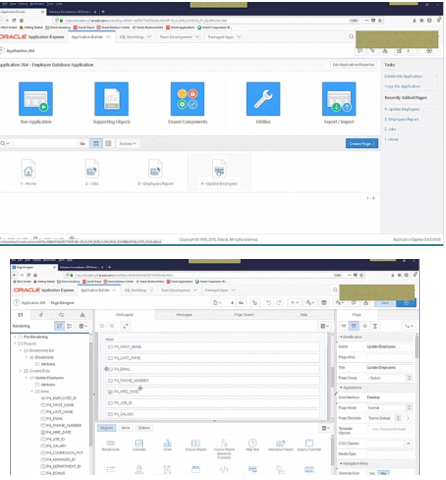
\includegraphics[width=8cm]{image/t.PNG}}
    \end{figure}
   \newpage  \item Setelah ini, buka halaman untuk mengoding, sebelum itu buka department id
    \begin{figure}[h]
        \centerline{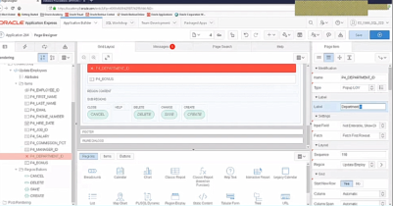
\includegraphics[width=8cm]{image/u.PNG}}
    \end{figure}
    \item setelah kedua table menjoin, jangan lupa mengoding  di SQL queri untuk mengecek seperti SELECT first_name from employees Jika  teruning  dengan baik maka berhasil.
    \begin{figure}[h]
        \newpage \centerline{\includegraphics[width=8cm]{image/v.PNG}}
    \end{figure}
\end{enumerate}
\end{enumerate}
\end{enumerate}
\end{document}
